\documentclass[tikz,border=8pt]{standalone}
\usepackage{amsmath,amssymb}
\usetikzlibrary{arrows.meta,calc}

\begin{document}
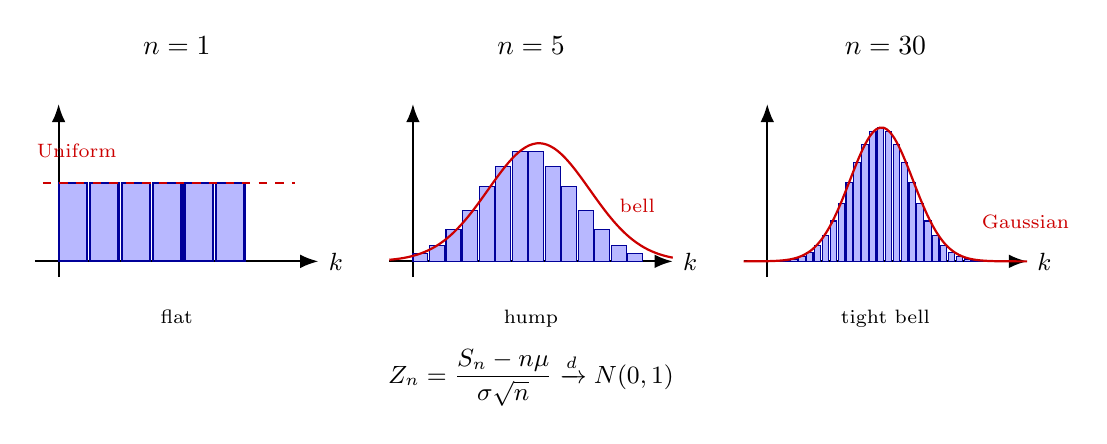
\begin{tikzpicture}[>=Latex]

  % n = 1 (uniform)
  \begin{scope}[xshift=0cm]
    \node[font=\bfseries, anchor=south] at (1.5, 2.5) {$n=1$};
    \draw[->, thick] (-0.3, 0) -- (3.3, 0) node[right, font=\small]{$k$};
    \draw[->, thick] (0, -0.2) -- (0, 2.0);

    \foreach \k in {1,...,6}{
      \pgfmathsetmacro{\bx}{(\k-1)*0.4}
      \filldraw[blue!28, draw=blue!60!black, thick] (\bx, 0) rectangle ({\bx+0.36}, 1.0);
    }
    \draw[red!80!black, thick, dashed] (-0.2, 1.0) -- (3.0, 1.0);
    \node[font=\scriptsize, red!80!black, anchor=west] at (-0.4, 1.4) {Uniform};
    \node[font=\scriptsize, anchor=north] at (1.5, -0.5) {flat};
  \end{scope}

  % n = 5 (triangular, hint of bell)
  \begin{scope}[xshift=4.5cm]
    \node[font=\bfseries, anchor=south] at (1.5, 2.5) {$n=5$};
    \draw[->, thick] (-0.3, 0) -- (3.3, 0) node[right, font=\small]{$k$};
    \draw[->, thick] (0, -0.2) -- (0, 2.0);

    \foreach \k/\h in {1/0.10, 2/0.20, 3/0.40, 4/0.65, 5/0.95, 6/1.20, 7/1.40, 8/1.40, 9/1.20, 10/0.95, 11/0.65, 12/0.40, 13/0.20, 14/0.10}{
      \pgfmathsetmacro{\bx}{(\k-1)*0.21}
      \filldraw[blue!28, draw=blue!60!black, thin] (\bx, 0) rectangle ({\bx+0.19}, \h);
    }
    \draw[red!80!black, thick, smooth, samples=80, domain=-0.3:3.3]
      plot(\x, {1.5*exp(-(\x-1.6)*(\x-1.6)*1.2)});
    \node[font=\scriptsize, red!80!black, anchor=west] at (2.5, 0.7) {bell};
    \node[font=\scriptsize, anchor=north] at (1.5, -0.5) {hump};
  \end{scope}

  % n = 30 (sharp gaussian)
  \begin{scope}[xshift=9.0cm]
    \node[font=\bfseries, anchor=south] at (1.5, 2.5) {$n=30$};
    \draw[->, thick] (-0.3, 0) -- (3.3, 0) node[right, font=\small]{$k$};
    \draw[->, thick] (0, -0.2) -- (0, 2.0);

    \foreach \k in {1,...,30}{
      \pgfmathsetmacro{\bx}{(\k-1)*0.10}
      \pgfmathsetmacro{\h}{1.7*exp(-((\k-15)*(\k-15))/30)}
      \filldraw[blue!28, draw=blue!60!black, thin] (\bx, 0) rectangle ({\bx+0.08}, \h);
    }
    \draw[red!80!black, thick, smooth, samples=80, domain=-0.3:3.3]
      plot(\x, {1.7*exp(-((\x-1.45)*(\x-1.45))/0.32)});
    \node[font=\scriptsize, red!80!black, anchor=west] at (2.6, 0.5) {Gaussian};
    \node[font=\scriptsize, anchor=north] at (1.5, -0.5) {tight bell};
  \end{scope}

  % bottom equation
  \node[font=\small, anchor=north] at (6, -1.0)
    {$Z_n=\dfrac{S_n - n\mu}{\sigma\sqrt n}\xrightarrow{d}N(0,1)$};
\end{tikzpicture}
\end{document}
